\chapter{Implementation}
\label{implementation}
Here, we present implementation details in the developed software. Its functionality is described on a selected example. More implementation details can be found on CD in the generated doxygen~\cite{doxygen} documentation. We will use the following example to describe optimizations and plan generation:


\begin{verbatim}
select
    l_orderkey,
    sum(l_extendedprice*(1-l_discount)) as revenue,
    o_orderdate,
    o_shippriority
from
    customer,
    orders,
    lineitem
where
    c_mktsegment = '[SEGMENT]'
    and c_custkey = o_custkey
    and l_orderkey = o_orderkey
    and o_orderdate < date '[DATE]'
    and l_shipdate > date '[DATE]'
group by
    l_orderkey,
    o_orderdate,
    o_shippriority
order by
    revenue desc,
    o_orderdate;
\end{verbatim}

This example was taken from TPC benchmark TM H~\cite{benchmark}. Parameters $[DATE]$ and $[SEGMENT]$ are constants. Tables do not contain any indices in this benchmark. Columns starting with \verb|o_| are from the table \verb|order|, columns beginning with \verb|l_| are from the table \verb|lineitem| and columns with prefix \verb|c_| belong to the table \verb|customers|.



\section{Input}

The input is XML file containing logical query plan. In this section, we describe its structure. 

\subsection{Sort}

The root of every algebra tree contains the sort operator, even if the output does not have to be sorted. In this case, sort has empty parameters. The following example displays the sort operator structure:


\lstset{
  language=XML,
  morekeywords={encoding,
    xs:schema,xs:element,xs:complexType,xs:sequence,xs:attribute}
}
\begin{lstlisting}
<?xml version="1.0" encoding="utf-8"?>
<sort xmlns:xsi="http://www.w3.org/2001/XMLSchema-instance"
 xsi:noNamespaceSchemaLocation="algebra.xsd">
  <parameters>
    <parameter column="revenue" direction="desc" />
    <parameter column="o_orderdate" direction="asc" />
  </parameters>
  <input>
  ...
  <input>
</sort>
\end{lstlisting}

The sort is the root element of XML file. Inside the $<$parameters$>$ element, we can find sort parameters specifying columns and the sort order. This example represents sort $\tau_{revenue:desc,o\_orderdate:asc}(...)$. The element $<$input$>$ should contain other algebra tree node.

\subsection{Group}

Next example shows the group node:

\begin{lstlisting}
<group>
  <parameters>
    <group_by column="l_orderkey"/>
    <group_by column="o_orderdate" />
    <group_by column="o_shippriority"/>
    <sum argument="x" output="revenue"/>
  </parameters>
  <input>
  ...
  <input>
</group>
\end{lstlisting}

This node represents expression $\gamma_{l\_orderkey,o\_orderdate,o\_shippriority,x=sum(x)}(...)$. Group element must have at least one $<$group\_by$>$  parameter or at least one aggregate function.  Another algebra operator should be inside the element $<$input$>$.

\subsection{Selection}

The selection is presented in the following example:

\begin{lstlisting}

<selection>
  <parameters>
    <condition>
      <lower>
        <constant type="date" value="today"/>
        <column name="l_shipdate"/>
      </lower>
    </condition>
  </parameters>
  <input>
  ...
  </input>
</selection>
\end{lstlisting}
This example represents the following expression: $\sigma_{today<l\_shipdate}$. The $<$condition$>$ element can contain multiple conditions connected by $<$and$>$ or $<$or$>$ elements. Input algebra supports operators $=$, $<$ and $\leq$.  Only $<$column$>$ or $<$constant$>$ element can be present in the leafs of the expression tree. Possible call of a boolean function from the selection is presented in the following example:

\begin{lstlisting}
<condition>
  <boolean_predicate name="like">
    <argument>
      <column name="x"/>
    </argument>
    <argument>
      <constant type="int" value="445" />
    </argument>
  </boolean_predicate>
</condition>
\end{lstlisting}

Used boolean predicate has to be supported by runtime (Bobox operators). The compiler does not check if called predicate does exist.

\subsection{Join}

The join operator without condition represents cross join. We can use join with multiple equal conditions or with one simple unequal condition. The first example contains equal conditions:

\begin{lstlisting}
<join>
  <parameters>
    <equal_condition>
      <equals>
        <column name="a"/>
        <column name="b"/>
      </equals>
      <equals>
        <column name="c"/>
        <column name="d"/>
      </equals>
    </equal_condition>
    <column name="a" input="first"/>
    <column name="b" input="second"/>
    <column name="c" input="first"/>
    <column name="d" input="second" newName="e" />
  </parameters>
<input>
...
</input>
\end{lstlisting}

This example represents join with condition $a=b~and~c=d$. In join equal condition, the first column has to be from the first relation and the second column comes from the second relation. The columns $a$ and $c$ are from the first input and $b$ and $d$ are from the other one. Joins do not copy all columns to the output. We have to specify non--empty sequence of output columns. For every column we have to provide the name and the input number. We can also rename the join output column by using the attribute $newName$. In the last example we renamed the output column $d$ to $e$.

The next example shows join with inequality condition:

\begin{lstlisting}
<join>
  <parameters>
    <less_condition>
      <and>
        <lower_or_equals>
          <column name="a1"/>
          <column name="b"/>
        </lower_or_equals>
      <lower_or_equals>
        <column name="b"/>
        <column name="a2"/>
      </lower_or_equals>
    </and>
  </less_condition>
  <column name="a1" input="first"/>
  <column name="b" input="second"/>
  <column name="a2" input="first"/>
</parameters>
<input>
...
</input>
</join>
\end{lstlisting}
This example represents join with the condition $a1\leq b\leq a2$. First element $<$lower\_or\_equals$>$ has to contain the column from the first relation followed by the column from the second relation. On the other hand, the second element $<$lower\_or\_equals$>$ must have these columns in the reversed order. The element $<$lower\_or\_equals$>$ can be replaced by the element $<$lower$>$. The rules for specifying the output column are the same as in the join with equal conditions. The element $<$input$>$ should contain two algebra operators.

\subsection{Anti--join}

\begin{lstlisting}
<antijoin>
  <parameters>
    <equal_condition>
      <equals>
        <column name="d"/>
        <column name="b"/>
      </equals>
    </equal_condition>
    <column name="d"/>
  </parameters>
<input>
...
<input>
</antijoin>
\end{lstlisting}

This is an example of anti--join with the simple condition $d=b$. The structure is almost the same as join with equal conditions. We can output columns only from the first relation and these columns can be renamed.
\\
\subsection{Table}
Table operator is the leaf of the algebra tree. We specify here the name of read table, its columns and indices. The number of rows can be given in order to get a better plan. If we do not have that information, we assume that a table has 1000 tuples. For every column we have to specify its name and type. Other optional parameter is $number\_of\_unique\_values$ which is important for estimating the size of join. If this information is missing, we will assume that $number\_of\_unique\_values$ is the size of the table to the power of $\frac{4}{5}$. This assumption is only experimental since the number of unique values comes from the interval $\langle 0, table~size\rangle$. There are two types of indices: clustered and  unclustered. Every table can have only one clustered index. For each index, we have to provide the attribute names and the sort order. The following example contains the table algebra node:
 
\begin{lstlisting}
<table name="orders" numberOfRows="1500000">
  <column name="o_orderdate" type="int"/>
  <column name="o_shippriority" 
  type="int" number_of_unique_values="30000"/>
  <column name="o_orderkey" type="int"/>
  <column name="o_custkey" type="int" />
  <index type="clustered" name="index">
    <column name="o_orderdate" order="asc" />
    <column name="o_shippriority" order="asc" />
  </index>
</table>
\end{lstlisting}

\subsection{Union}
The union operator does not have any parameters and the columns from both inputs must have the same names. Example:
\begin{lstlisting}
<union>
  <input>
  ...
  </input>
</union>
\end{lstlisting}

\subsection{Extended projection}
The following example of an extended projection represents expression \\ $\pi_{l\_orderkey,o\_orderdate,o\_shippriority,x=l\_extendedprice*(1-l\_discount)}(...)$:
\begin{lstlisting}
<column_operations>
  <parameters>
    <column name="l_orderkey"></column>
    <column name="o_orderdate"></column>
    <column name="o_shippriority"></column>
    <column name="x">
      <equals>
        <times>
          <column name="l_extendedprice"/>
          <minus>
            <constant type="double" value="1"/>
            <column name="l_discount"/>
          </minus>
        </times>
      </equals>
    </column>
  </parameters>
  <input>
  ...
  </input>
</column_operations>
\end{lstlisting}

The extended projection contains a list of columns. Newly computed columns contain element $<$equals$>$ with expression. Expression tree can contain arbitrary function call which has to be supported by Bobox operators. Function call is explained in the following example:


\begin{lstlisting}
<column_operations>
  <parameters>
    <column name="x">
      <equals>
        <aritmetic_function name ="sqrt" returnType="double">
          <argument>
            <constant type="double" value="2"/>
          </argument>
        </aritmetic_function>
      </equals>
    </column>
  </parameters>
  <input>
    ...
  </input>
</column_operations>
\end{lstlisting}
 
Last example computes new column named $x$ with values $\sqrt{2}$.
 
\section{Building relational algebra tree} 

In this section, we describe the construction of logical plan as well as the structure for its storage. Relational algebra operators are represented by children of the abstract class \texttt{AlgebraNodeBase}. It has the following abstract subclasses:
\begin{itemize}

\item \texttt{UnaryAlgebraNodeBase} -- abstract class for algebra operator with one input.

\item \texttt{BinaryAlgebraNodeBase}  -- abstract class for algebra operator with two inputs.

\item \texttt{GroupedAlgebraNode} -- abstract class for algebra operator with the variable number of inputs.

\item \texttt{NullaryAlgebraNodeBase} --  abstract class for algebra tree leafs.

\end{itemize}

All algebra operators are children of one of the mentioned classes. Every operator has pointer to its parent and smart pointers to its children, if they exist. 

Expressions in algebra nodes are represented by polymorphic trees. All expression nodes are children of the class \texttt{Expression}.

We used the visitor pattern for manipulating and reading expression and algebra tree. All nodes (algebra and expression) contain the method \texttt{accept} which calls visitor method on the class \texttt{AlgebraVisitor}/\texttt{ExpressionVisitor}. All classes, which manipulate the algebra tree, are children of class \texttt{AlgebraVisitor}.


\begin{figure}[h!]
  \centering
    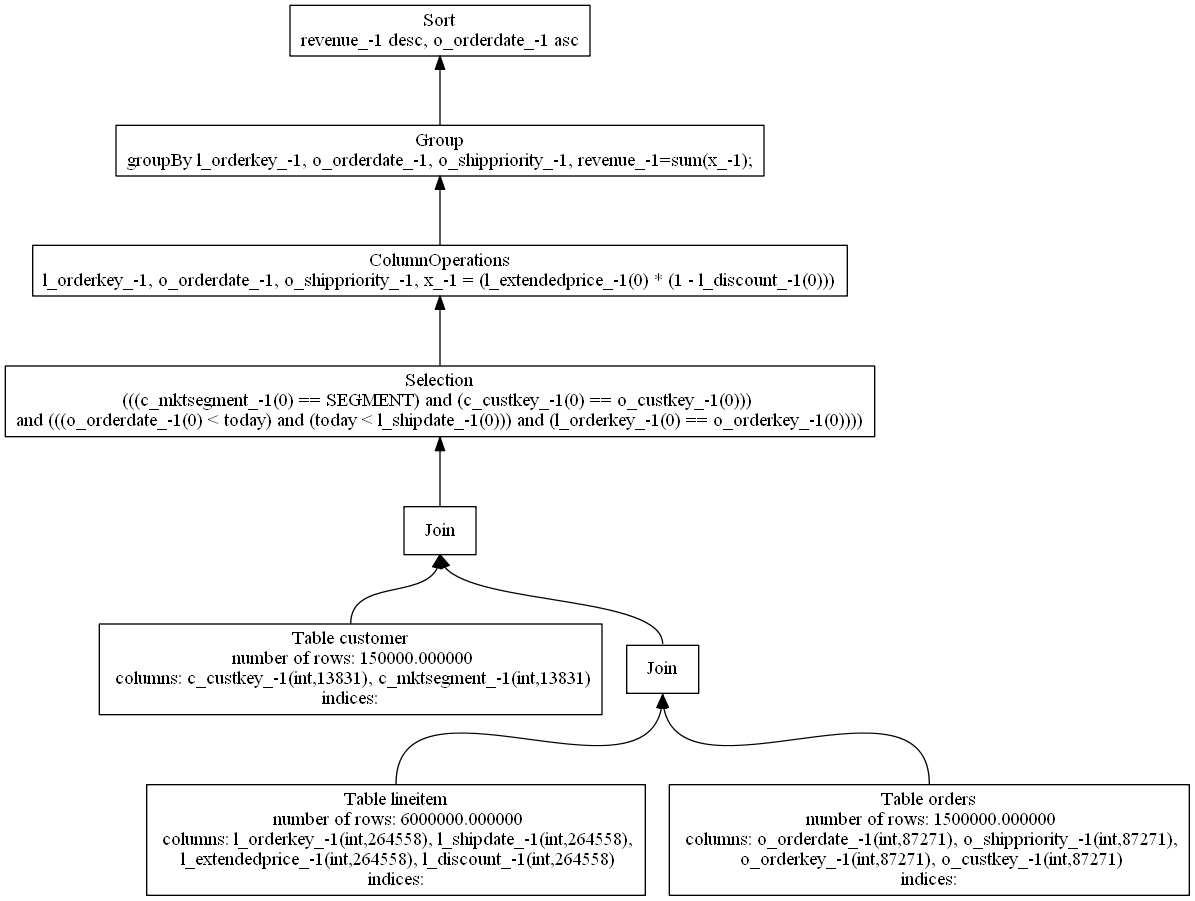
\includegraphics[width=1.0\textwidth]{algebratree1}

      \caption{Example of algebra tree.}
          \label{fig:algebratree1}
\end{figure}

In Figure~\ref{fig:algebratree1} we presented the example of algebra tree of the query presented in the beginning of this chapter. We have transformed it to cross joins of three tables. After cross joins we applied selection with condition located in the \verb|where| clause. The obtained result was used to compute new column and to apply grouping operator computing aggregate functions. Output of the query was sorted. In table reading operator, we can see additional information like the name of the table. Every attribute has the suffix $\_-1$ which is the unique identifier of the column. After the algebra tree is built from XML, the unique identifiers are not assigned and they contain default value $-1$. The inputs, from which the columns originate, are represented by the numbers in parentheses. Input operators are numbered from $0$. All columns in used selection come from the zeroth input.

We used library Xerces version 3.1.1~\cite{xerces} for parsing and validating the input XML file. It parses the input file and creates the DOM tree. This tree has to be validated against XML schema. Parsing and validation of XML is performed in the class \texttt{XmlHandler}.

Every algebra tree has to have the sort operator on the top. We call \texttt{Sort} constructor with root element as an argument. This method copies all the information from DOM tree and calls the method \texttt{AlgebraNodeBase::constructChildren} which decides what constructor to call on children of processed node. This way we recursively build the algebra tree.



\section{Semantic analysis and node grouping}

Semantic checking is processed by the class \texttt{SemanticChecker}, which checks if columns used in expressions exist and if the output columns of each operator have unique name. During this checking we assign unique identifier to every column. After this phase, we do not need attribute names anymore, we use only the unique identifiers.

Logical plan is visited by \texttt{GroupingVisitor}. In this phase, joins represented by the class \texttt{Join} are replaced by the grouped join represented by the class \texttt{GroupedJoin} with two or more input relations. We apply \texttt{GroupingExpressionVisitor} on every expression. The \texttt{GroupingExpressionVisitor} groups expressions with $and$ and $or$ operators. This step simplifies splitting condition into sub conditions.

\section{Algebra optimization}

We need to prepare logical tree for optimizing it by pushing down selections. To do this, we split selection into smaller conditions using the rule:
\begin{itemize}
\item $\sigma_{A~and~B}(R)=\sigma_{A}(\sigma_{B}(R))$
\end{itemize}
A chain of selections is created from every selection. This operation performed by \texttt{SelectionSpitingVisitor}.

Afterwards, we apply \texttt{SelectionColectingVisitor} which stores pointers of all selections in the relational algebra tree. These pointers are input into \texttt{Push\-Selection\-Down\-Visitor}. It pushes all selections down the tree as much as possible and also converts cross joins into regular joins if we have selection with equal condition.
\begin{figure}[h!]
  \centering
    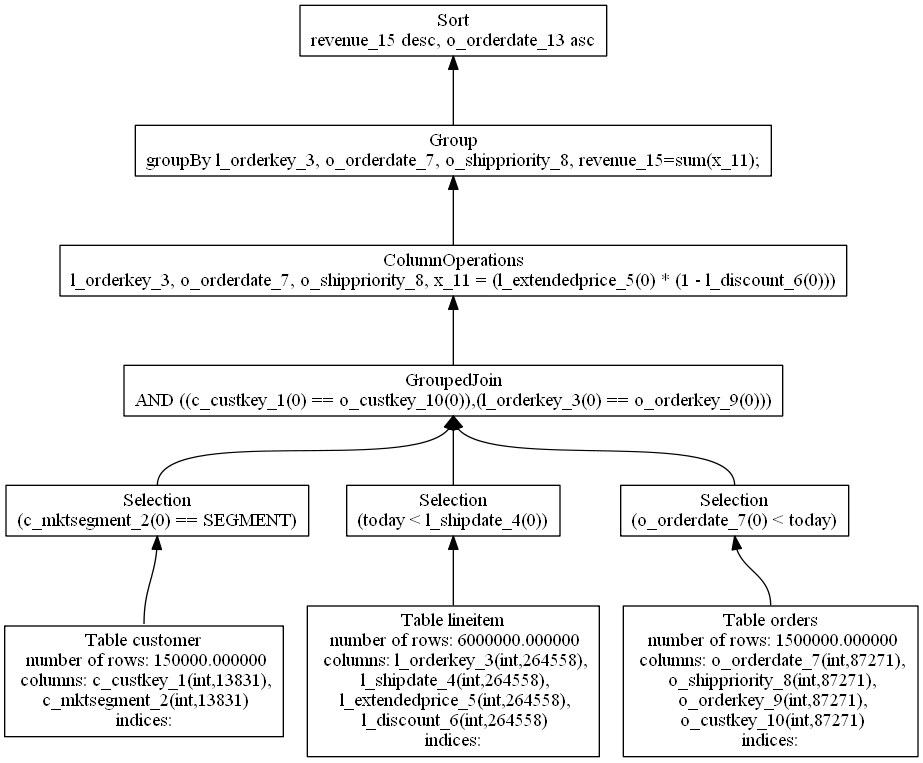
\includegraphics[width=1.0\textwidth]{algebratree2}

      \caption{Example of optimized algebra tree.}
          \label{fig:algebratree2}
\end{figure}
At this moment, we have optimized tree but it still contains the selection chains. To resolve this problem, we apply \texttt{SelectionFusingVisitor} that applies the following rule to the tree:
\begin{itemize}
\item $\sigma_{A}(\sigma_{B}(R))=\sigma_{A~and~B}(R)$
\end{itemize}

Optimized algebra tree is depicted in Figure~\ref{fig:algebratree2}. Contrary to the case of Figure~\ref{fig:algebratree1}, this tree has grouped join with three input relations. The selection above joins was split and moved down the tree. Some parts of the condition became parts of the join condition, others were pushed down to one of the branches of grouped join. It can be seen that new tree has columns with assigned unique identifiers which eliminate the need of the input number for each column.

This output is optimized algebra tree. Needless to say, more optimizations can be implemented in order to improve logical plan.

\section{Generating plan}

Final logical plan will be processed by \texttt{AlgebraCompiler} which outputs $n$ best plans. Parameter $n$ is a constant in  \texttt{AlgebraCompiler} represented by variable \texttt{NUM\-BER\_\-OF\_\-PLANS}. 

This visitor visits node of algebra tree, then it calls itself on its children. We use generated plans for child nodes to create plans for the current node. After that, we store the best plans in the variable \texttt{result}, relation size in the variable \texttt{size} and output columns in the variable \texttt{outputColumns}. 

For each algebra node we generate all possible algorithms. Generated plans are stored in the variable \texttt{result}. This variable stores a max--heap, where plans are compared by their overall time complexity. This time complexity is computed as a sum of time complexities in all physical operators in the current plan. Maximal size of the heap is $n$. If there are more than $n$ plans in the heap, we remove plan in the root of the heap.

Both join order algorithms can be found in the method \texttt{visitGroupedJoin}. If the number of join relations is smaller than $k$, we use the dynamic programing algorithm to estimate order of join. If we have more relations to join, we use the greedy algorithm. Constant $k$ is represented in the variable \texttt{LI\-MIT\_\-FOR\_\-GREEDY\_\-JOIN\_\-ORDER\_\-ALGORITHM}. Both join algorithms call the method \texttt{join} which combines plans and generates all possible plans.


Physical plan is represented as polymorphic tree. 


\begin{figure}[h!]
  \centering
    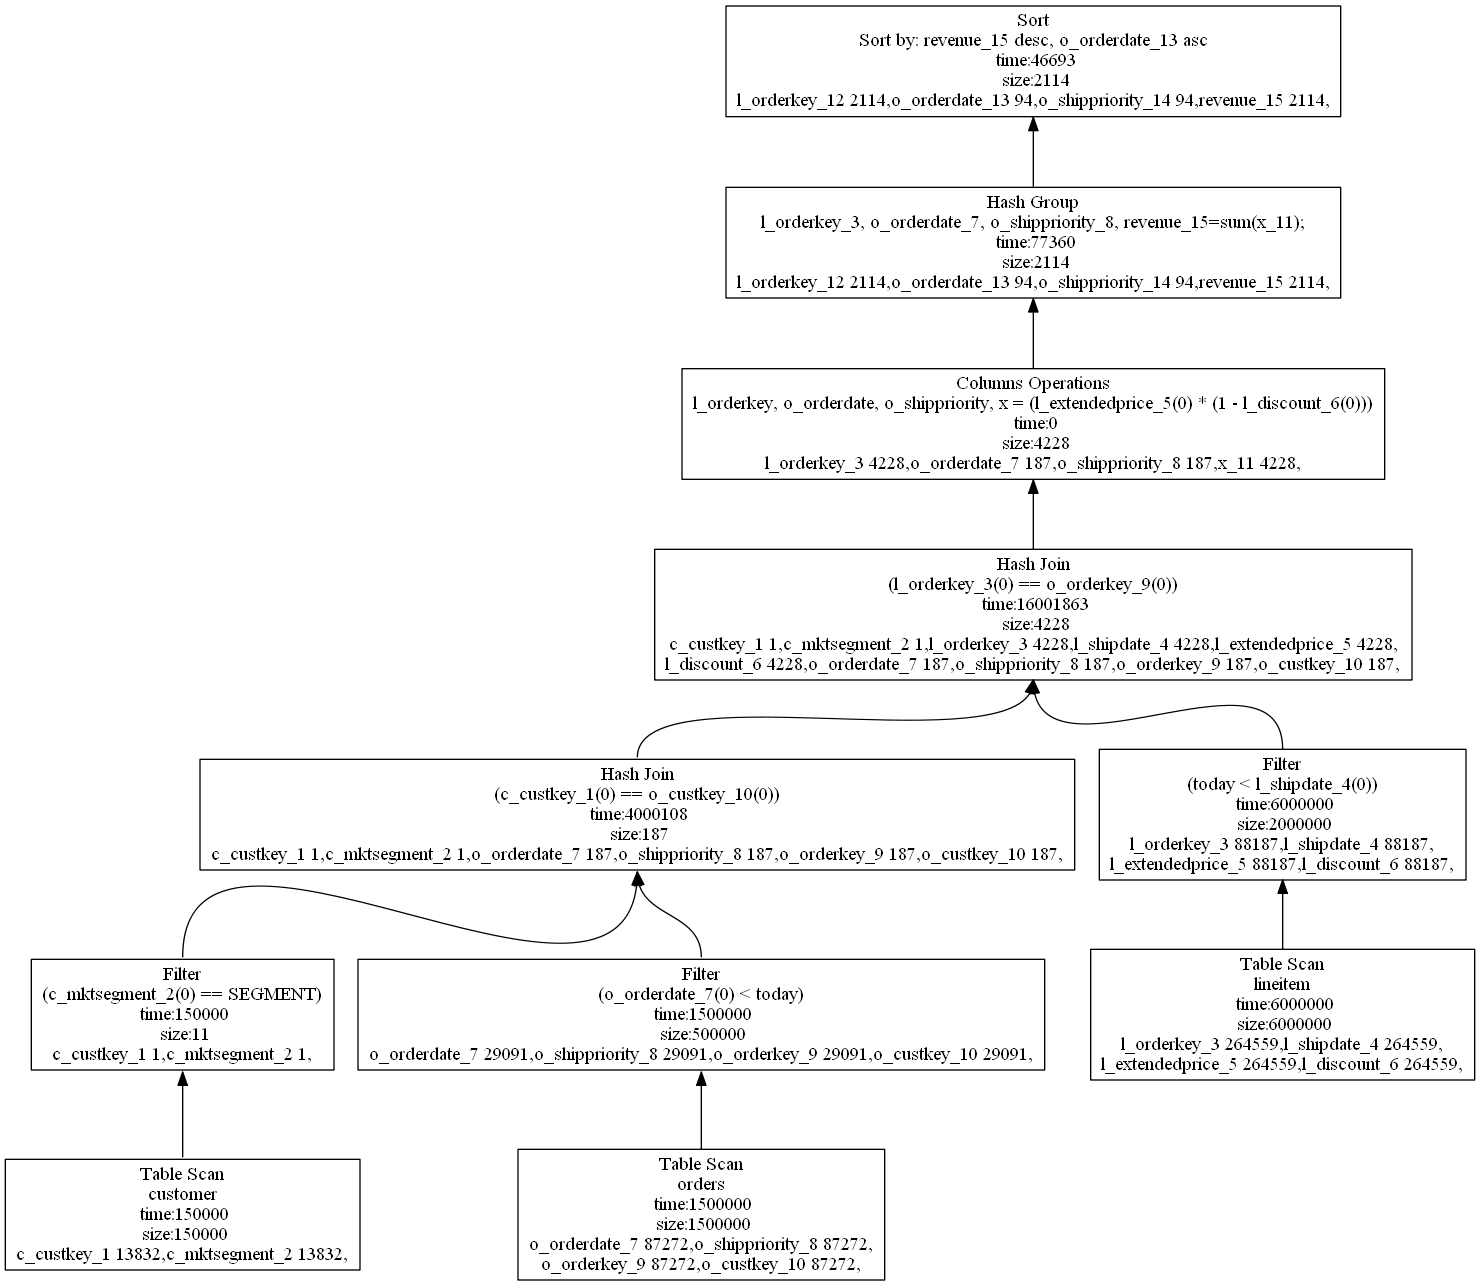
\includegraphics[width=1.0\textwidth]{physicalplan}

      \caption{Example of physical plan.}
          \label{fig:physicalplan}
\end{figure}


The best generated physical plan for query presented in the beginning of this chapter is drawn in Figure \ref{fig:physicalplan}. Each operator contains estimated size and run time. Output columns with their unique identifiers and estimated number of unique values are given on the bottom of the physical operators. Since read tables do not contain any indices we have to read all the tables and filter the results. After that, we can only use hash join because sorting relations for merge join would be to expensive and nested loop join is not supported by runtime or compiler. From the result we compute new columns and use the hash group algorithm. We did not use sorted group as input is not sorted and output has to be sorted by other than group column.

Physical operators are chosen according to their estimated time complexity which is computed from the estimated size of relation. In the class \texttt{TimeComplexity}, we have static functions which compute time complexity for each operation. It also contains constants used in these functions. We assume that this constants or whole functions need to be improved. This improvement can be achieved in the future if the tests and measurements of the evaluation queries in Bobox are performed. At the time of submitting this thesis, the runtime environment is not fully functional.




\section{Resolving sort parameters}

Sort parameters structure in Figure~\ref{fig:sortparameters} is represented by the class \texttt{Possible\-Sort\-Parameters}. Every group of columns is stored in the class \texttt{SortParameters}. The class \texttt{SortParameter} is used to store column name and sort direction.


We take generated plans from the class \texttt{AlgebraCompiler}. Sort parameters of sort nodes need to be resolved. Two plans also can contain the same physical operator. Hence, we need to clone plans in order to assure that no algorithm object is used in two or more plans.

We used \texttt{CloningPhysicalOperatorVisitor} for cloning and we resolve generated plans in \texttt{SortResolvingPhysicalOperatorVisitor}. Physical plan with unresolved sort parameters can be seen in Figure~\ref{fig:plansortunresolved}.
\begin{figure}[h!]
  \centering
    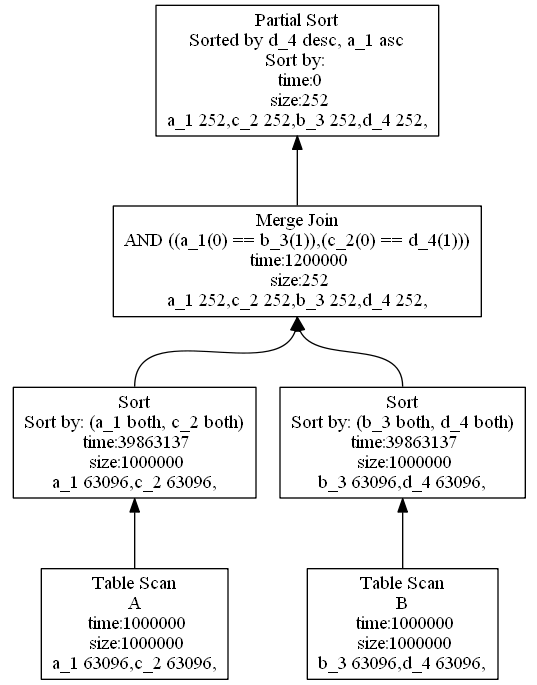
\includegraphics[width=0.6\textwidth]{plansortunresolved}

      \caption{Example of physical plan.}
          \label{fig:plansortunresolved}
\end{figure}
\noindent
It contains two sort algorithms. Left one has the following possible parameters:

\begin{itemize}
\item $a:both, c:both$
\item $c:both, a:both$
\end{itemize}
Right sort algorithm has these sort parameters:
\begin{itemize}
\item $b:both, d:both$
\item $d:both, b:both$
\end{itemize}

At the time of generating this algorithm, we did not know what order was the best to choose. After merge join, the plan has to be sorted by $d:desc,a:asc$. At the top of the tree, we generated partial sort which does not do anything because relation is already sorted. It only indicates that we choose $d:desc,a:asc$ from all sort parameter possibilities and we do not have to do any additional sorting.

\texttt{SortResolvingPhysicalOperatorVisitor} works down the tree. Variable \texttt{sortParameters} is used for storage of information how the input of current node was sorted. We adjust sort parameters of the sort algorithm using this variable. The adjusted plan is drawn in Figure~\ref{fig:plansortresolved}.

\begin{figure}[h!]
  \centering
    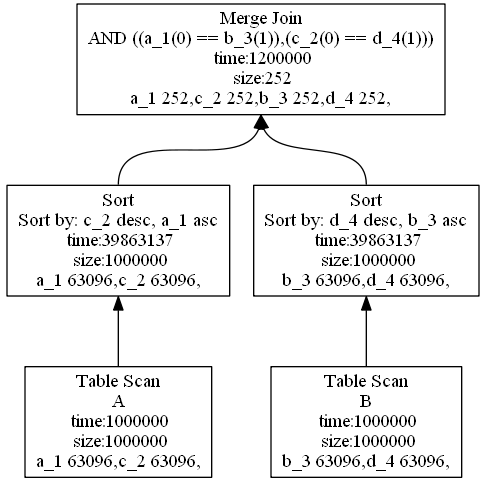
\includegraphics[width=0.6\textwidth]{plansortresolved}

      \caption{Example of final physical plan.}
          \label{fig:plansortresolved}
\end{figure}

Output of the query has to be sorted by $d:desc,a:asc$. Visitor sets that input of partial sort has to be sorted by $d:desc,a:asc$. In the merge join we compute that left input has to be sorted by $c:desc,a:asc$ and right input has to be sorted by $d:desc,b:asc$. We choose correct sort parameters in the sort algorithms using this information. 
There can be situations where we use sort based algorithm but output does not have to be sorted and thus we can choose arbitrary order of sort parameters. 


\section{Output}

 Output in Bobolang is generated by \texttt{Bobox\-Plan\-Writing\-Physical\-Operator\-Vi\-si\-tor}. We can also generate output from the algebra tree. Visitor \texttt{Graph\-Drawing\-Visitor} can generate output in dot language. Output of physical plan can be written in dot language using \texttt{Physical\-Operator\-Drawing\-Visitor}. \texttt{Physical\-Operator\-Drawing\-Visitor\-WithouSorts} provides dot output without partial sorts with empty sort parameters. In the following sections, we present text output generated by the implemented compiler.

\subsection{Filters}
Example: 
\begin{lstlisting}
Filter(double,double,int)->(double,double,int)
f(condition="OP_LOWER(OP_double_CONSTANT(4.8),1)"); 
\end{lstlisting}

Input and output columns are the same and they are both numbered from $0$.
This filter operator takes input of two double streams and integer stream and it filters by condition $4.8<(column~1)$. Columns $0$ and $1$ are streams of doubles and column $2$ is stream of integers. We have also another version of this operator which guarantees that the input and the output are sorted in the same way. In order to use it, we write $FilterKeepingOrder$ instead of $Filter$ in the operator declaration. 

\subsection{Group}
Example: 
\begin{lstlisting}
HashGroup(string,string,int)->(string,int,int)
g(groupBy="1",functions="count(),max(2)");
\end{lstlisting}
Input columns are numbered from $0$. Output columns consist of grouped columns and computed aggregate functions in the same order as specified in parameters. 
This example groups by column $1$ and computes aggregate functions $COUNT$ and $MAX$. The parameter of the function $MAX$ is column $2$. 

We have also sorted version of this operator. It assumes that input is sorted by group columns. In order to use it, we write $SortedGroup$ instead of $HashGroup$ in the declaration.

\subsection{Column operations}
Example: 
\begin{lstlisting} 
ColumnsOperations(int,int,int,int,int)->(int,int,int,double)
c(out="0,3,4,OP_TIMES(2,OP_MINUS(OP_double_CONSTANT(1),2))"); 
\end{lstlisting}
Input columns are numbered from $0$. Output is specified in the parameter $out$. If it contains the number of column, it copies input to output, otherwise it computes a new column. 
This example copies columns labeled with $0,3,4$ to output and computes a new column with the expression: $(column~2)*(1-(column~2))$.

\subsection{Cross join}
Example:
\begin{lstlisting} 
CrossJoin(string,int),(int,string)->(string,string)
c(left="0,1",right="2,3",out="0,3");
\end{lstlisting}
Parameters $left$ and $right$ specify how the columns are numbered from the first and second input, respectively. The join outputs only the columns given in the $out$ argument. 

The other join operators have the same $left$, $right$ and $out$ parameters. The last mentioned rule applies to the following operators:
\begin{itemize}
\item \texttt{Hash join}
\item \texttt{Merge equi-join}
\item \texttt{Hash anti-join}
\item \texttt{Merge anti-join}
\end{itemize} 

\subsection{Hash join}
Example:
\begin{lstlisting}
HashJoin(int,int),(int,int,int,int)->(int,int,int,int,int,int)
h(left="0,1",right="2,3,4,5",out="0,1,2,3,4,5",
leftPartOfCondition="0,1","rightPartOfCondition="5,2"); 
\end{lstlisting}
This operator works only with equal condition which is given in the parameters $leftPartOfCondition$ and $rightPartOfCondition$. Relation in the first input should be stored in a hash table since its estimated size is smaller than the size of the second relation. This example computes join with the condition:\\
 $(column~0=column~5)~and~(column~1=column~2)$.

\subsection{Merge equi--join}
Example:
\begin{lstlisting}
MergeEquiJoin(int),(int)->(int,int))
m(left="0",right="1",out="0,1",leftPartOfCondition="0:D",
rightPartOfCondition="1:D");
\end{lstlisting}
Condition is given in the parameters $left\-Part\-Of\-Con\-di\-tion$ and $right\-Part\-Of\-Con\-di\-tion$, and these parameters contain information about the sorting of the inputs. This example computes join with condition $(column~0 = column~1)$. The first input is sorted by the column $0$ descending and the second input is sorted by the column~$1$ descending.

\subsection{Merge non equi--join}
Example:
\begin{lstlisting}
MergeNonEquiJoin(date,date),(date)->(date,date,date)
m(left="0,1",right="2",out="0,1,2",
leftInputSortedBy = "0:A,1:A",rightInputSortedBy = "2:A",
condition="OP_AND(OP_LOWER_OR_EQUAL(0,2)
,OP_LOWER_OR_EQUAL(2,1))");
\end{lstlisting}

This operator joins sorted relations. Numbering of columns from the first and second input is specified in the $left$ and $right$ parameter, respectively. Parameters $leftInputSortedBy$ and $rightInputSortedBy$ store information about the sorting of the input relations. Join condition is in the parameter $condition$. Operator in this example joins by condition $column~0 \leq column~2\leq column~1$. The first input is sorted by the column $0$ ascending and the column $1$ ascending and the second input is sorted by the column $2$ ascending.

\subsection{Hash anti--join}
Example:
\begin{lstlisting}
HashAntiJoin(int),(int)->(int)
h(left="0",right="1",out="0",leftPartOfCondition="0",
rightPartOfCondition="1"); 
\end{lstlisting}

Parameter $out$ can only contain columns from the first input. Condition is given in the parameters $leftPartOfCondition$ and $rightPartOfCondition$.
Relation in the first input should be stored in the hash table since its estimated size is smaller than the size of the second relation. This example computes the anti--join with the condition $(column~0==column~1)$.

\subsection{Merge anti--join}
Example:
\begin{lstlisting}
MergeAntiJoin(int),(int)->(int)
m(left="0",right="1",out="0",leftPartOfCondition="0:D",
rightPartOfCondition="1:D");
\end{lstlisting}

The operator copies to the output only the rows from the first input for which no row in the second input satisfying given condition exists.
Condition is given in the parameters $leftPartOfCondition$ and $rightPartOfCondition$ and they also contain information about the sorting of inputs. This example computes join with the condition $(column~0==column~1)$. The first input is sorted by the column $0$ descending and the second input is sorted by the column $1$ descending.

\subsection{Table scan}
Example:
\begin{lstlisting}
TableScan()->(int,int,int,int)
t(name="lineitem",
columns="l_orderkey,l_shipdate,l_extendedprice,l_discount");
\end{lstlisting}
This operator scans the table specified in the parameter $name$ and reads only columns given in the parameter $columns$.

\subsection{Scan And Sort By Index}
Example:
\begin{lstlisting}
ScanAndSortByIndexScan()->(string,string,int)
s(name="people",index="index",
columns="user_name,country,parameter"); 
\end{lstlisting}
Scan And Sort operator reads the whole table given in the $name$ using the $index$ and reads the columns specified in the attribute $columns$.

\subsection{Index Scan}

Example:
\begin{lstlisting}
IndexScan()->(int,int)
i(name="customer",index="index2",columns="c_custkey,c_mktsegment",
condition="OP_EQUALS(1,OP_string_CONSTANT(SEGMENT))");
\end{lstlisting}
Index Scan operator reads part of the table given in the $name$ using the $index$ and reads the columns specified in the attribute $columns$. Operator reads only the rows satisfying the condition given in the attribute $condtion$.



\subsection{Sort}
Example:
\begin{lstlisting}
SortOperator(int,int)->(int,int)
s(sortedBy="0",sortBy="1:D");
\end{lstlisting}
Input and output columns are the same and they are numbered from $0$. Parameter $sortedBy$ specifies by which columns is the table sorted and parameter $sortBy$ specifies by which columns should the table be sorted. Example is already sorted by the column~$0$ and will be sorted by the column $1$ descending.


\subsection{Union}
Example:
\begin{lstlisting}
Union(int,string)(string,int)->(int,string)
u(left="0,1",right="1,0",out="0,1");
\end{lstlisting}
Numbering of columns from the first input is given in the $left$ parameter. Second input uses the same number of columns as the first output. This information is specified in the parameter $right$. Operator appends the rows from the input $1$ to the rows from input $0$. The order of the output columns is specified in the parameter $out$. Operator unites columns with the same numbers.

